% 可并入总论文；所需宏包与数值宏见 main.tex。
\section{问题一：交会定位区域的构建与直径计算}
单次示向测量只能约束干扰源所在的方向区间，无法唯一确定其位置。本章将有界示向误差转化为平面几何约束，通过不同检测位置的观测构建公共定位区域，并计算该区域的最大空间跨度。在此基础上，进一步判断以区域直径为直径构造的圆能否覆盖全部候选位置，为后续精确定位与清除提供依据。

\subsection{示向误差几何模型}
以目标圆域中心 $O$ 为原点建立平面直角坐标系，$x$ 轴正向向东，$y$ 轴正向向北，坐标单位为米。方位角以正东方向为零度，逆时针为正。设第 $i$ 个检测点为 $S_i=(x_i,y_i)$，同一频道的示向读数为 $\theta_i$。由于测向误差上界为 $\varepsilon=1^\circ$，真实方位角 $\varphi_i$ 满足
\begin{equation}
 \theta_i-\varepsilon\leq\varphi_i\leq\theta_i+\varepsilon.
\end{equation}
上述区间按圆周角理解；跨越 $0^\circ$ 时，应将角度连续展开或采用模 $360^\circ$ 的等价判定。定义两条边界射线的单位方向向量
\begin{equation}
 \boldsymbol u_i^- = \begin{pmatrix}\cos(\theta_i-\varepsilon)\\\sin(\theta_i-\varepsilon)\end{pmatrix},\qquad
 \boldsymbol u_i^+ = \begin{pmatrix}\cos(\theta_i+\varepsilon)\\\sin(\theta_i+\varepsilon)\end{pmatrix}.
\end{equation}
其中三角函数计算时将角度转换为弧度。记二维叉积为 $\boldsymbol a\times\boldsymbol b=a_xb_y-a_yb_x$，则一次测向对应的可行扇区为
\begin{equation}
 W_i=\{P:\boldsymbol u_i^-\times(P-S_i)\geq0,\quad
 \boldsymbol u_i^+\times(P-S_i)\leq0\}.
\end{equation}
因此，可行位置位于两条边界射线之间，而非仅在示向中心线上。由于同一地点的测量误差在一段时间内保持不变，本模型不通过同点重复测量求平均来消除误差，而是利用不同位置的几何交会缩小候选范围。

本章遵循问题一程序的默认设定，仅使用示向角和目标圆域约束，不叠加有效接收半径及 $5\,\mathrm m$ 近场盲区。因而这里得到的是该建模口径下的候选区域；与完整物理约束下的候选集合应作区分。

\subsection{交会定位区域构建}
已知干扰源位于半径为 $1800\,\mathrm m$ 的目标圆域内，即
\begin{equation}
 B_0=\{(x,y):x^2+y^2\leq1800^2\}.
\end{equation}
同一干扰源的位置必须同时满足全部测向约束，故公共定位区域为
\begin{equation}\boxed{\Omega=B_0\cap\bigcap_{i=1}^{m}W_i.}\label{eq:intersection}\end{equation}
采用增量求交方式，令 $\Omega_0=B_0$，依次计算
\begin{equation}
 \Omega_i=\Omega_{i-1}\cap W_i,\quad i=1,2,\ldots,m.
\end{equation}
由集合交运算可知 $\Omega_i\subseteq\Omega_{i-1}$，故新增观测不会扩大定位区域。但区域缩小程度取决于各检测点的空间构型，不能保证每次观测均带来严格收缩。

数值实现采用 Shapely 进行几何布尔运算。目标圆每象限离散为 64 段，形成 256 边形；扇区外圆弧默认采用 65 个采样点。因此，程序输出是连续几何区域的多边形近似，记为 $\widehat\Omega$。为将无限扇区转化为有限几何对象，设置截断距离
\begin{equation}
 L_i=\|S_i-O\|+1800+1.
\end{equation}
对于任意 $P\in B_0$，由三角不等式得 $\|P-S_i\|\leq1800+\|S_i-O\|<L_i$，故理想扇区的截断不排除目标圆域内的点。折线离散仍存在近似误差，不能将其等同于解析圆弧运算。
若某次交集为空，或面积不超过 $10^{-8}\,\mathrm{m}^2$，程序报告公共区域为空或退化；其中退化情形不必然意味着观测矛盾，也可能是交集维数降低。

\begin{figure}[htbp]\centering
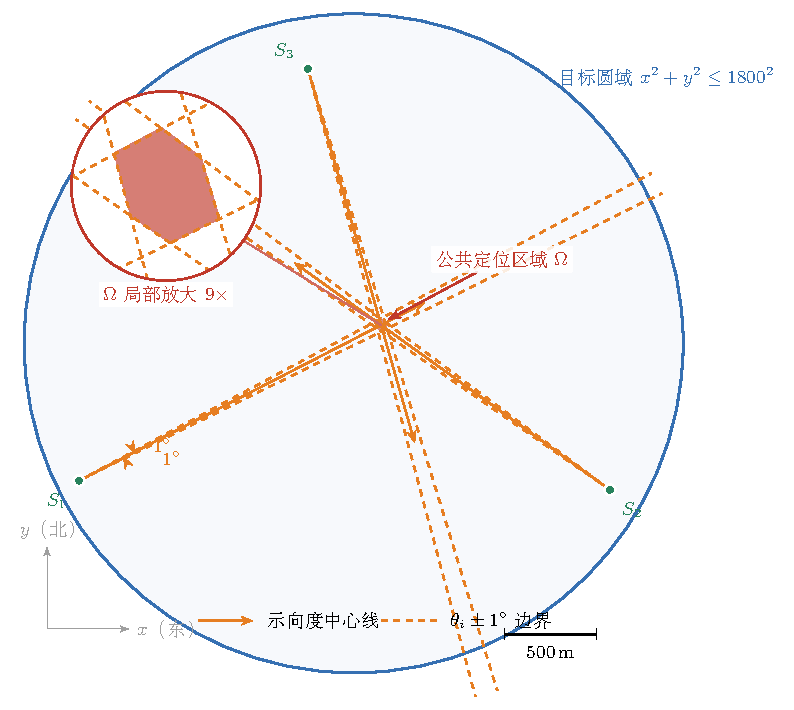
\includegraphics[width=.83\linewidth]{figures/intersection.pdf}
\caption{多点示向误差扇区及交会定位区域示意图（局部放大 $9$ 倍，误差角取 $1^\circ$）}\label{fig:intersection}
\end{figure}

\begin{quote}\small
\textbf{区域构建算法：}输入同一频道测向数据与误差上界；初始化 $\widehat\Omega\leftarrow\widehat B_0$；依检测顺序构造扇区多边形并更新 $\widehat\Omega\leftarrow\widehat\Omega\cap\widehat W_i$；若交集为空或面积不超过阈值则报告异常，否则输出最终定位多边形。
\end{quote}

\subsection{定位区域直径计算}
区域直径刻画任意两种候选位置之间可能出现的最大距离，定义为
\begin{equation}
 D=\operatorname{diam}(\Omega)=\max_{P,Q\in\Omega}\|P-Q\|_2.
\end{equation}
设 $H=\operatorname{Conv}(\Omega)$。任取凸包内两点 $X=\sum_i\alpha_iP_i$、$Y=\sum_j\beta_jQ_j$，其中 $P_i,Q_j\in\Omega$，系数非负且分别求和为 1，则
\begin{equation}
 \|X-Y\|_2=\left\|\sum_{i,j}\alpha_i\beta_j(P_i-Q_j)\right\|_2
 \leq\sum_{i,j}\alpha_i\beta_j\|P_i-Q_j\|_2\leq D.
\end{equation}
结合 $\Omega\subseteq H$，可得 $\operatorname{diam}(H)=\operatorname{diam}(\Omega)$。对于数值多边形，其凸包中的任一点均为凸包顶点的凸组合，同理可知最远点对能够在凸包顶点中取得。

设数值凸包顶点为 $P_1,\ldots,P_h$，则计算
\begin{equation}
 (A,B)\in\operatorname*{arg\,max}_{1\leq i<j\leq h}\|P_i-P_j\|_2,\qquad
 \widehat D=\|A-B\|_2.
\end{equation}
后文算例中的直径均指计算得到的 $\widehat D$，为简洁仍记作 $D$。当前程序采用凸包顶点两两枚举，共比较 $h(h-1)/2$ 组距离，直径搜索的时间复杂度为 $O(h^2)$，存储顶点所需额外空间为 $O(h)$。这不等同于寻找多边形最长边，因为最远点对可能是两个不相邻顶点。

本章默认约束的交集本身为凸集，凸包操作主要用于统一几何处理流程与提取候选极点。图\ref{fig:hull}以不规则凸多边形说明枚举过程，不引入虚构实验数值。
\begin{figure}[htbp]\centering\begin{tikzpicture}[scale=.9,>=Stealth]
\coordinate (A) at (-3,-.5);\coordinate (B) at (3,.4);
\filldraw[fill=red!12,draw=blue!65!black,thick] (A)--(-1.7,1.5)--(1.2,1.7)--(B)--(1.5,-1.4)--(-1.7,-1.5)--cycle;
\draw[gray,dashed] (-1.7,1.5)--(1.5,-1.4) (1.2,1.7)--(-1.7,-1.5);
\draw[red!70!black,very thick] (A)--(B) node[midway,above,sloped] {$D=\|A-B\|_2$};
\foreach \p in {(-3,-.5),(-1.7,1.5),(1.2,1.7),(3,.4),(1.5,-1.4),(-1.7,-1.5)} {\fill \p circle (2pt);}
\node[left] at (A) {$A$};\node[right] at (B) {$B$};\node at (0,-.8) {$\Omega=H$};
\end{tikzpicture}

\caption{定位区域凸包及最远点对示意图（原理示意）}\label{fig:hull}\end{figure}
\begin{quote}\small
\textbf{直径搜索算法：}求定位多边形的凸包并提取 $h$ 个顶点；初始化 $D=0$；对 $i=1,\ldots,h-1$ 以及 $j=i+1,\ldots,h$，计算 $d_{ij}=\|P_i-P_j\|_2$；当 $d_{ij}>D$ 时更新 $D$ 及端点 $A=P_i,B=P_j$；最终返回 $D,A,B$。
\end{quote}

\subsection{直径圆覆盖性分析}
由直径端点构造圆盘
\begin{equation}
 \mathcal C=\{P:\|P-C\|_2\leq D/2\},\qquad C=(A+B)/2.
\end{equation}
端点 $A,B$ 必然位于圆周上，但这不能证明其他候选点也在圆内。对定位多边形的全部边界顶点 $P_k$ 检查
\begin{equation}
 \|P_k-C\|_2\leq D/2+\tau,\qquad
 \tau=\max(10^{-9}\,\mathrm m,10^{-10}D).
 \label{eq:cover}
\end{equation}
圆盘是凸集，若所有顶点均在圆盘内，其凸组合也在圆盘内，因而整个多边形被覆盖；反之，只要一个顶点位于圆外，即可否定覆盖性。在忽略数值容差时，由恒等式
\begin{equation}
 (P_k-A)\cdot(P_k-B)=\|P_k-C\|_2^2-D^2/4
\end{equation}
可得等价的泰勒斯圆判据 $(P_k-A)\cdot(P_k-B)\leq0$。加入距离容差后，点积判据的右端相应变为 $D\tau+\tau^2$。这里的容差用于控制浮点舍入影响，不代表圆弧离散误差的上界。

\textbf{直径圆并不一定覆盖整个定位区域。}以边长为 $D$ 的等边三角形为例，其区域直径也为 $D$。选择任一边 $AB$ 构造直径圆，第三个顶点 $P$ 到边中点的距离为
\begin{equation}
 \|P-C\|_2=\frac{\sqrt3}{2}D>\frac D2,
\end{equation}
故 $P$ 位于圆外。相较之下，矩形以对角线为直径构造的圆能够覆盖整个矩形，如图\ref{fig:cover}所示。该反例否定的是一般性的必然覆盖命题；程序对每个具体区域仍需独立判断，而不能始终返回否定结果。直径圆也不应直接称为最小覆盖圆。
\begin{figure}[htbp]\centering\begin{tikzpicture}[scale=.85]
\begin{scope}[xshift=-3.2cm]
\draw[blue!65!black,dashed,thick] (0,0) circle (1.8);
\filldraw[fill=red!12,draw=red!65!black] (-1.44,-1.08) rectangle (1.44,1.08);
\draw[thick] (-1.44,-1.08)--(1.44,1.08) node[midway,above left] {$C$};
\fill (0,0) circle (1.6pt);
\node[below left] at (-1.44,-1.08) {$A$};\node[above right] at (1.44,1.08) {$B$};
\node at (-.8,-.3) {$D$};\node at (.8,.25) {$D/2$};
\node at (0,-2.5) {(a) 可以覆盖};
\end{scope}
\begin{scope}[xshift=3.2cm]
\draw[blue!65!black,dashed,thick] (0,0) circle (1.25);
\filldraw[fill=red!12,draw=red!65!black] (-1.25,0)--(1.25,0)--(0,2.165)--cycle;
\draw[thick] (-1.25,0)--(1.25,0) node[midway,below=12pt] {$D$};
\draw[purple,dashed] (0,0)--(0,2.165);
\fill (0,0) circle (1.6pt);\node[below] at (0,0) {$C$};
\node[left] at (-1.25,0) {$A$};\node[right] at (1.25,0) {$B$};
\fill[purple] (0,2.165) circle (2.5pt);\node[above,purple] at (0,2.165) {$P$};
\node[right,font=\small] at (.1,1.55) {$\frac{\sqrt3 D}{2}>\frac D2$};
\node at (0,-2.5) {(b) 不能覆盖};
\end{scope}
\end{tikzpicture}

\caption{定位区域直径圆覆盖性的两种情形}\label{fig:cover}\end{figure}

\subsection{算例与结果分析}
选取仓库运行日志 \texttt{P3\_run\_log.jsonl} 中频道 4 的前三个不同检测位置，记录位于日志第 5、77、79 行。三条记录均为已接受且返回示向度的测量响应，属于同一运行中同一频道的观测。此处仅作为日志算例展示几何算法，不将其视为独立正式评测结论。输入及由问题一求解函数计算的结果分别见表\ref{tab:input}、表\ref{tab:result}。表中输入坐标保留八位小数以便复核，实际计算使用原始日志精度。
\begin{table}[htbp]\centering\caption{主算例测向输入数据}\label{tab:input}\begin{tabular}{crrrc}\toprule 检测点 & $x_i/\mathrm m$ & $y_i/\mathrm m$ & $\theta_i/(^\circ)$ & 误差范围\\\midrule
$S_1$ & 0.00000000 & 0.00000000 & 186.06 & $\pm1^\circ$ \\
$S_2$ & -845.15139195 & -403.18365019 & 95.97 & $\pm1^\circ$ \\
$S_3$ & -877.29411572 & -93.23217920 & 122.92 & $\pm1^\circ$ \\
\bottomrule\end{tabular}\par\smallskip{\small 数据来源：仓库 \texttt{P3\_run\_log.jsonl}，频道 4，按顺序选取前三个不同检测位置；计算使用日志原始精度。}\end{table}
\begin{table}[htbp]\centering\caption{主算例计算结果}\label{tab:result}\begin{tabular}{lr}\toprule 指标 & 数值\\\midrule
定位区域面积 / $\mathrm{m}^2$ & 2.97 \\
边界顶点数 & 3 \\
直径 $D$ / $\mathrm m$ & 13.53 \\
端点 $A$ / $\mathrm m$ & $(-877.29, -93.23)$ \\
端点 $B$ / $\mathrm m$ & $(-884.45, -81.75)$ \\
圆心 $C$ / $\mathrm m$ & $(-880.87, -87.49)$ \\
半径 $D/2$ / $\mathrm m$ & 6.76 \\
直径圆是否覆盖 & 是 \\
\bottomrule\end{tabular}\end{table}

依次加入三次观测后，候选区域面积分别为 $\FirstArea\,\mathrm{m}^2$、$\SecondArea\,\mathrm{m}^2$ 和 $\FinalArea\,\mathrm{m}^2$。可见，不同位置的测向约束交会后，狭长扇区逐渐收缩为小范围候选区域。最终区域有三个边界顶点，直径为 $D=\CaseDiameter\,\mathrm m$，表示最不利方向上的最大空间不确定尺度。
\begin{figure}[htbp]\centering
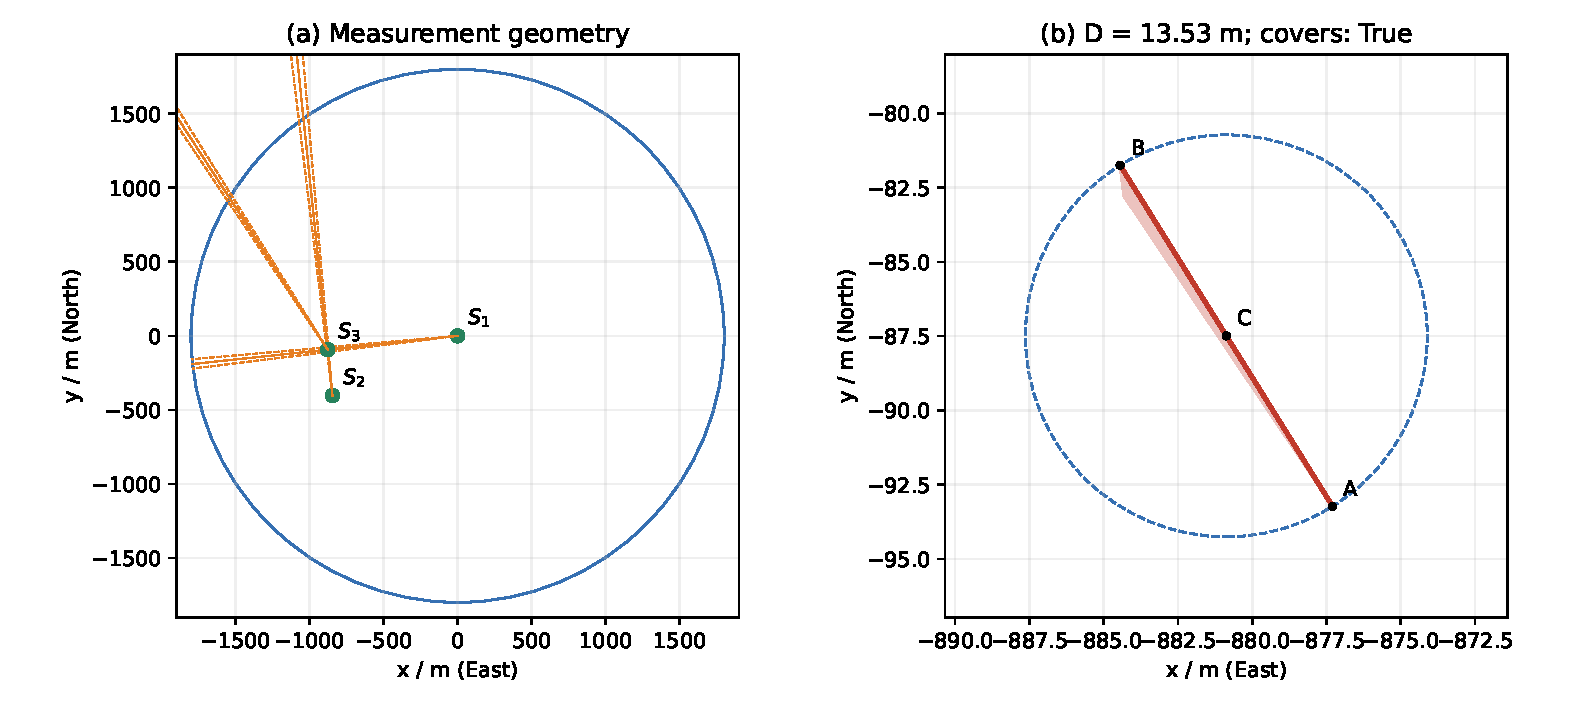
\includegraphics[width=\linewidth]{figures/case.pdf}
\caption{主算例定位区域、区域直径及直径圆：左图为全域测向构型，右图为定位区域放大图}\label{fig:case}\end{figure}
本算例的全部顶点通过式\eqref{eq:cover}的检验，直径圆能够覆盖数值定位区域，其半径为 $\CaseRadius\,\mathrm m$，小于清除半径 $20\,\mathrm m$。因此，在本章几何模型和数值精度下，以圆心 $C$ 为清除位置满足覆盖要求。一般情况下，不能仅凭 $D\leq40\,\mathrm m$ 就作出相同判断，还必须确认候选区域被相应圆覆盖。

值得注意的是，本算例中端点 $A$ 与第三检测位置重合，这是默认模型保留扇区顶点、未剔除近场盲区的结果，并非断言干扰源位于检测点。本章未开展圆弧离散精度敏感性实验，因此不对默认离散参数的收敛精度作额外结论。

\subsection{问题一结论}
通过将 $\pm1^\circ$ 示向误差转化为扇区约束，并与目标圆域进行增量求交，得到同一干扰源的定位可行区域；随后对数值区域的凸包顶点进行两两距离比较，获得区域直径及一组端点。图\ref{fig:intersection}展示了多点观测的信息融合过程，表\ref{tab:result}给出了日志算例的可复核结果。

区域直径刻画最大空间不确定性，但以该直径构造的圆并不必然覆盖全部候选位置，图\ref{fig:cover}给出了明确反例。以直径端点中点为圆心、以 $D/2$ 为半径时，仍须检验全部边界顶点。上述区域、直径端点、圆心与覆盖结论可作为后续检测点选择和清除策略的几何基础。
